\chapter{Numerical Algebra -- Approximating Roots}
In this chapter we want to solve equations using a computer.  Consider the equation
$\ell(x) = r(x)$ (where $\ell$ and $r$ stand for left and right respectively).  To solve
this equation we can first rewrite it by subtracting the right-hand side from the left to
get
\[ \ell(x) - r(x) = 0. \]
For example, if we want to solve $\sin(x) + 9 = x^2 - \tan(x)$ then this is the same as
solving $(\sin(x) + 9 ) - (x^2 - \tan(x)) = 0$ (please don't try to solve this one by
hand!).  Hence, we can write $f(x)=\ell(x)-r(x)$
and observe that every algebraic equation can be written as
\[ \text{if } f(x) = 0 \quad \text{find } x. \]

\begin{figure}[ht!]
    \begin{center}
        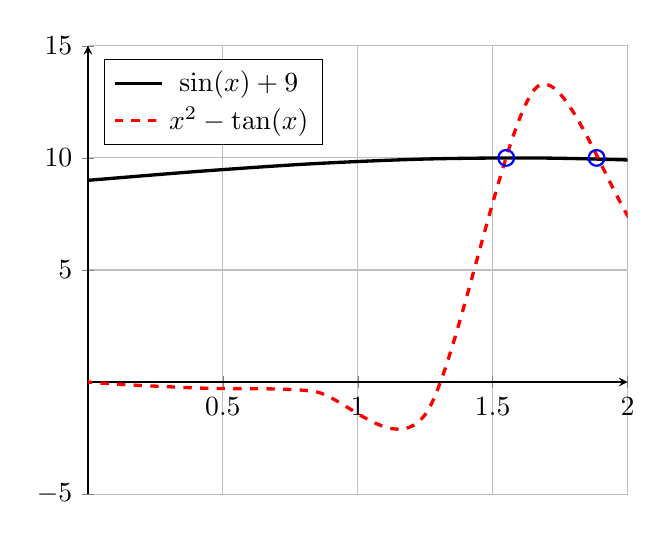
\begin{tikzpicture}
            \begin{axis}[axis lines=center, grid, xmin=0, xmax=2, ymin=-5, ymax=15, legend
                pos=north west]
                \addplot[black, smooth, very thick] {sin(deg(x)) + 9};
                \addlegendentry{$\sin(x) + 9$};
                \addplot[red, smooth, dashed, very thick] {x^2 - tan(deg(x))};
                \addlegendentry{$x^2-\tan(x)$};
                \draw[thick, blue] (axis cs:1.55,10) circle(0.1cm);
                \draw[thick, blue] (axis cs:1.885,10) circle(0.1cm);
            \end{axis}
        \end{tikzpicture}
        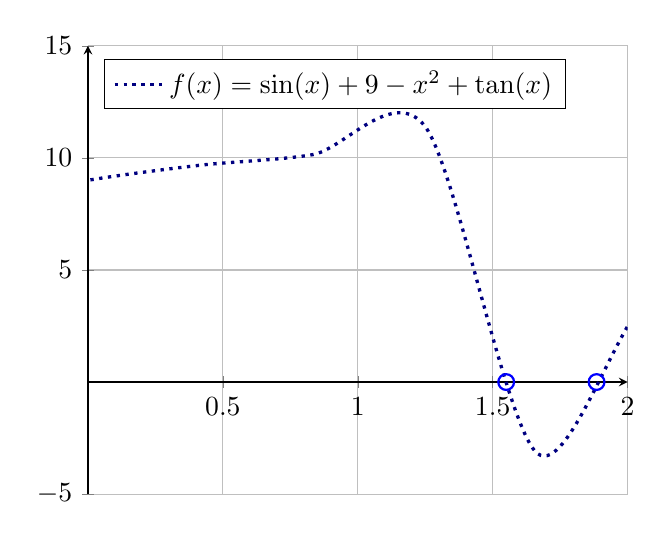
\begin{tikzpicture}
            \begin{axis}[axis lines=center, grid, xmin=0, xmax=2, ymin=-5, ymax=15, legend
                pos=north west]
                \addplot[blue!50!black, dotted, smooth, very thick] {sin(deg(x)) + 9 - x^2 + tan(deg(x))};
                \addlegendentry{$f(x) = \sin(x) + 9 - x^2+\tan(x)$};
                \draw[thick, blue] (axis cs:1.55,0) circle(0.1cm);
                \draw[thick, blue] (axis cs:1.885,0) circle(0.1cm);
            \end{axis}
        \end{tikzpicture}
    \end{center}
    \caption{The left-hand plot shows two nonlinear functions, $\ell(x) = \sin(x) + 9$ and
        $r(x) = x^2 - \tan(x)$, with their intersection points marked. The right-hand plot
    shows the equivalent problem formed by solving $\ell(x) - r(x) = 0$.}
    \label{fig:initial_root_example}
\end{figure}

We now have one way to view every algebraic equation-solving problem.  As we'll see in
this chapter, if $f(x)$ has certain properties then different numberical techniques for
solving the equation will apply.

\section{The Bisection Method}

\begin{thm}[The Intermediate Value Theorem]
    If $f$ is a continuous function on the closed interval $[a,b]$ and $y_*$ lies between
    $f(a)$ and $f(b)$, then there is a point $x \in [a,b]$ where $f(x) = y_*$.
    \label{thm:IVT}
\end{thm}


\begin{problem}
    Draw a picture of what the intermediate value theorem says graphically.
\end{problem}
\solution{
Draw a continuous function that crosses the line $y=y_*$ on the interval $[a,b]$.
}

\begin{problem}
    If $y_*=0$ the intermediate value theorem gives us important information about solving
    equations.  What does it tell us?
\end{problem}
\solution{
If $y_*=0$ and $f(x)$ is continuous then we know that there is a solution to the algebraic
equation $f(x) = 0$.
}


The following (partial) algorithm, known as the Bisection Method, uses the Intermediate
Value Theorem to systematically approximate solutions to the algebraic equation $f(x) =
0$.
\begin{algorithm}[The Bisection Method]
    Assume that $f(x)$ is continuous on the interval $[a,b]$. To make approximations of
    the solutions to the equation $f(x) = 0$, do the following:
    \begin{enumerate}
        \item Check to see if $f(a)$ and $f(b)$ have opposite signs
            (why is this important?).\solution{In order for the IVT to apply you must have
            $0$ in between $f(a)$ and $f(b)$.}
        \item Compute the midpoint $m=(a+b)/2$ and evaluate $f(m)$.
        \item Compare the signs of $f(a)$ vs $f(m)$ and $f(b)$ vs $f(m)$.  Replace one of
            the endpoints with $m=(a+b)/2$. Which one do you replace and why?
            \solution{Replace the endpoint where the function has the same sign as
                $f(m)$}
        \item Repeat steps 2 and 3
        \item Stop when $f(m)$ is {\it close enough} to zero.
    \end{enumerate}
\end{algorithm}

\begin{problem}
    Draw a picture illustrating what the Bisection Method does to approximate solutions to
    the algebraic equation $f(x) = 0$.
\end{problem}


\begin{problem}
    Write a MATLAB function for the Bisection Method, and write a test script
   that verifies that your function works properly. Be sure that it can take an
    anonymous function handle as an input along with an initial lower bound, an initial
    upper bound, and an optional error tolerance. The output should be only 1 single number: the
    root.\\
    \texttt{function root=Bisection(f , a , b , tol)}
\end{problem}

\begin{problem}
    Test your Bisection Method code on the following algebraic equations.
    \begin{enumerate}
        \item $x^2 - 2 = 0$ on $x \in [0,2]$ \solution{$\sqrt{2} \approx 1.414$}
        \item $\sin(x) + x^2 = 2\ln(x) + 5$ on $x \in [0,5]$ (be careful! make a plot
            first) \solution{$0.0860$ and $2.4953$ }
        \item $(5-x)e^{x}=5$ on $x \in [0,5]$\solution{$4.9651$}
    \end{enumerate}
\end{problem}


\begin{problem}
    Let $f(x)$ be a continuous function on the interval $[a,b]$ and assume that $f(a)
    \cdot f(b) <0$.  If we want to approximate the solution to the equation $f(x)=0$ to
    within $\delta$ how many iterations will the bisection method need? \\ Hint: If we
    want an approximation within $\delta$ then the width of the interval is $2\delta$.
\end{problem}
\solution{
    The width of the interval will always be half as large at each iteration.
    \begin{center}
        \begin{tabular}{|c|c|}
            \hline
            Iteration & Width of Interval \\ \hline \hline
            0 & $|a-b|$ \\
            1 & $\frac{|a-b|}{2}$ \\
            2 & $\frac{|a-b|}{2^2}$ \\
            \vdots & \vdots \\
            $k$ & $\frac{|a-b|}{2^k}$ \\
            \hline
        \end{tabular}
    \end{center}
    After $k$ steps the width of the interval is equal to $\frac{|a-b|}{2^k}$ so to reduce
    the interval to less than $2\delta$ we must have
    \[ \frac{|a-b|}{2^k} \le 2 \delta \implies \frac{|a-b|}{2\delta} \le 2^k \implies
        \frac{|a-b|}{\delta} \le 2^{k+1} \implies k \ge \log_2 \left(
        \frac{|a-b|}{\delta} \right) - 1 \]
}


\begin{problem}
    How many iterations of the bisection method are necessary to approximate $\sqrt{3}$ to
    within $10^{-3}$, $10^{-4}$, \dots, $10^{-15}$ using the initial interval
    $[a,b]=[0,2]$?
\end{problem}
\solution{
    \begin{center}
        \begin{tabular}{|c|c|}
            \hline
            Error & Num. Iterations \\ \hline \hline
            $10^{-3}$ & 10\\
            $10^{-4}$ & 14\\
            $10^{-5}$ & 17\\
            $10^{-6}$ & 20\\
            $10^{-7}$ & 24\\
            $10^{-8}$ & 27\\
            $10^{-9}$ & 30\\
            $10^{-10}$ & 34\\
            $10^{-11}$ & 37\\
            $10^{-12}$ & 40\\
            $10^{-13}$ & 44\\
            $10^{-14}$ & 47\\
            $10^{-15}$ & 50\\\hline
        \end{tabular}
    \end{center}
}



\section{The Regula Falsi Method}
The bisection method is one of many methods for performing root finding on a continuous
function.  The next algorithm takes a slightly different approach.

\begin{algorithm}[The Regula Falsi Method]
    Assume that $f(x)$ is continuous on the interval $[a,b]$. To make approximations of
    the solutions to the equation $f(x) = 0$, do the following:
    \begin{enumerate}
        \item Check to see if $f(a)$ and $f(b)$ have opposite signs so that the
            intermediate value theorem guarantees a root on the interval.
        \item Write the equation of the line connecting the points $(a,f(a))$ and
            $(b,f(b))$. Fill in the blanks in the point slope form.
            \[ y - \underline{\hspace{0.4in}} = \underline{\hspace{0.4in}} \cdot \left(
                x - \underline{\hspace{0.4in}} \right) \]
            \solution{
                \[ y - f(a) = \left( \frac{f(b) - f(a)}{b-a} \right) \left( x-a
                    \right) \]
            }
        \item Find the $x$ intercept of the linear function that you wrote in the previous
            step.
            \[ x = \underline{\hspace{2in}} \]
            \solution{
                \[ 0 - f(a) = \left( \frac{f(b) - f(a)}{b-a} \right) \left( x-a
                    \right) \implies x = a+ \left( \frac{-f(a) (b-a)}{f(b)-f(a)} \right) \]
            }
        \item Just as we did with the bisection method, compare the signs of $f(a)$ vs
            $f(c)$ and $f(b)$ vs $f(c)$.  Replace one of the endpoints with $c$. Which one
            do you replace and why?
            \solution{Replace the endpoint where the function has the same sign as
                $f(c)$}
        \item Repeat steps 2 - 4.
        \item Stop when $f(c)$ is {\it close enough} to zero.
    \end{enumerate}
\end{algorithm}

\begin{problem}
    Draw a picture of what the Regula Falsi method does to approximate a root.
\end{problem}


\begin{problem}
    Give sketches of functions where the Regula Falsi method will perform faster than the
    Bisection method and visa versa.  Justify your thinking with several pictures and be
    prepared to defend your answers.
\end{problem}
\solution{
    The Regula Falsi method will perform very fast if the root is {\it close} to one of
    the chosen endpoints.  The bisection method will perform very vast if the root is {\it
    close} to the midoint of the two chosen endpoints.
}

\begin{problem}
   Write a MATLAB function to implement the Regula Falsi method, and write a test script
   that verifies that your function works properly. Your function should accept an
    anonymous function handle as an input along with an initial lower bound, an initial
    upper bound, and an optional error tolerance. The output should be only 1 single number: the
    root.\\
    \texttt{function root=RegulaFalsi(f , a , b , tol)}
\end{problem}



\section{Newton's Method}
We now investigate a calculus-based method (originally proposed by Isaac Newton and later
modified by Joseph Raphson) for solving the algebraic equation $f(x)=0$. In very basic
terms, this method involves iteratively finding tangent lines to a differentiable curve
and locating where those tangent lines intersect the horizontal axis.
\begin{algorithm}[Newton's Method]
    The Newton-Raphson method for solving algebraic equations can be described as follows:
    \begin{enumerate}
        \item Check that $f$ is a twice differentiable function on a given domain and find
            a way to guarantee that $f$ has a root on that domain (this step happens by
            hand, not on the computer).
        \item Pick a starting point $x_0$ in the domain
        \item Write the equation of a tangent line to $f$ at $x_0$.  Fill in the blanks in
            the point-slope form.
            \[ y - \underline{\hspace{0.4in}} = \underline{\hspace{0.4in}} \cdot \left(
                x - \underline{\hspace{0.4in}} \right) \]
            \solution{
                \[ y - f(x_0) = f'(x_0) \left( x-x_0 \right) \]
            }
        \item Find the $x$ intercept of the equation of the tangent line and call this new
            point $x_1$.  
            \[ x_1 = \underline{\hspace{2in}} \]
            \solution{
                \[ x_1 = x_0 - \frac{f(x_0)}{f'(x_0)} \]
            }
        \item Now iterate the process by replacing the labels ``$x_1$'' and ``$x_0$'' in
            the previous step with $x_{n+1}$ and $x_{n}$.
            \[ x_{new} = \underline{\hspace{2in}} \]
            \solution{
                \[ x_{n+1} = x_{n} - \frac{f(x_n)}{f'(x_n)} \]
            }
        \item Iterate step 5 until $f(x_{n})$ is {\it close} to zero.
    \end{enumerate}
\end{algorithm}

\begin{problem}
    Draw a picture of what Newton's method does graphically.
\end{problem}

\begin{problem}
    There are several reasons why Newton's method could fail.  Work with your partners to
    come up with a list of all of the reasons.  Support each of your reasons with a
    sketch.
\end{problem}
\solution{
    Newton's method will fail if
    \begin{itemize}
        \item the slope at the initial guess is zero (leading to no intersections of the
            tangent line with the $x$-axis), 
        \item the slope at any point in the interval is undefined,
        \item the initial guess is {\it too far away} from the intended root.
    \end{itemize}
}

\begin{problem}
    Write a MATLAB function for Newton's method.  Your function needs to accept an
    anonymous function handle, the derivative of the anonymous function hand, an initial
    guess, and an optional error
    tolerance. The only output should be the solution to the equation that you are
    solving.  Write a test script to verify that your Newton's method code indeed works.
    \\
    \texttt{function soln = Newton(f , df , x0 , tol)}
\end{problem}


\begin{problem}\label{prob:newton_convergence}
    Newton's Method is known to have a {\it quadratic convergence rate}.  This means that 
    \[ \lim_{k \to \infty} \frac{|x_{k+1} - x_*|}{|x_k - x_*|^2} \]
    will be constant where $x_*$ is the roots that we're hunting for.  This implies that
    if we plot the error in the new iterate on the $y$-axis and the error in the old
    iterate on the $x$ axis of a log-log plot then we will see a constant slope of 2.
    (stop and verify why this would be true).
    
    In this problem we're going to build a numerical experiment to verify that Newton's
    method indeed has quadratic convergence.  Modify your Newton's method code so that it
    outputs all of the iterations instead of just the final root.  Once you have the
    iterations compute the error between the approximations and the exact root. For
    simplicity let's solve the equation $x^2-2=0$.  Plot the sequence of error
    approximations with the iterate $e_k$ on the $x$-axis and the iterate $e_{k+1}$ on the
    $y$-axis of a log-log plot.  \\ Your plot command will look something like: \\
    \texttt{loglog(error(1:end-1),error(2:end),'b*')} \\where \texttt{error} is a vector
    containing all of the errors.  Quadratic convergence means that at every iteration the
    error should decrease by roughly 2 orders of magnitude.  How can you see this in your
    plot?
\end{problem}


\begin{problem}
    Repeat the previous problem with the bisection and regula falsi
    methods.  Plot the errors of all three methods on the same plot and discuss the rates
    of convergence for the three methods.
\end{problem}


\section{Quasi-Newton Methods}
Newton's method requires that you have a function and a derivative of that function.  The
conundrum here is that sometimes the derivative is cumbersome or impossible to obtain but
you still want to have the great quadratic convergence exhibited by Newton's method.
Recall that Newton's method is
\[ x_{n+1} = x_n - \frac{f(x_n)}{f'(x_n)}. \]
If we replace $f'(x_n)$ with an approximation of the derivative then we may have a method
that is {\it close} to Newton's method in terms of convergence rate but is less
troublesome to compute. Any method that replaces the derivative in Newton's method with an
approximation is called a {\bf Quasi-Newton Method}.

\begin{algorithm}[Secant Method]
    To solve $f(x) = 0$:
    \begin{enumerate}
        \item Determine if there is a root {\it near} an arbitrary starting point $x_0$.
        \item Pick a second starting point {\it near} $x_0$. (Note: the points $x_0$ and
            $x_1$ should be close to each other.  The choice here is different than for
            the bisection method)
        \item Use the backward difference 
            \[ f'(x_n) \approx \frac{f(x_n) - f(x_{n-1})}{x_n - x_{n-1}} \]
            to approximate the derivative of $f$ at $x_n$.
        \item Perform the Newton-type iteration 
            \[ x_{n+1} = x_n - \frac{f(x_n)}{ \left(  \frac{f(x_n) - f(x_{n-1})}{x_n - x_{n-1}}\right)} \]
            until $f(x_n)$ is {\it close enough} to zero.  Notice that the new iteration
            simplifies to
            \[ x_{n+1} = x_n - \frac{f(x_n)\left( x_n - x_{n-1} \right)}{f(x_n) -
            f(x_{n-1})}. \]
    \end{enumerate}
\end{algorithm}

\begin{problem}
    Draw several pictures showing what the Secant method does pictorially.
\end{problem}

\begin{problem}
    Write MATLAB code for solving algebraic equations of the form $f(x) = 0$ with the
    Secant method.  Also write a test script that clearly shows that your code is working.
\end{problem}

\begin{problem}
    Choose a non-trivial algebraic equation for which you know the solution and write a
    script to empirically determine the convergence rate of the Secant method.  You may want to
    look back at \ref{prob:newton_convergence}.
\end{problem}


\begin{algorithm}[Steffensen's Method]
    To solve $f(x) = 0$:
    \begin{enumerate}
        \item Determine if there is a root {\it near} an arbitrary starting point $x_0$.
        \item In Steffensen's method we approximate the derivative with 
            \[ f'(x_n) \approx \frac{f(x_n + f(x_x)) - f(x_n)}{f(x_n)} \]
        \item Perform the Newton-type iteration 
            \[ x_{n+1} = x_n - \frac{f(x_n)}{ \left(  \frac{f(x_n + f(x_x)) - f(x_n)}{f(x_n)}\right)} \]
            until $f(x_n)$ is {\it close enough} to zero.  Notice that the new iteration
            simplifies to
            \[ x_{n+1} = x_n - \frac{f(x_n)^2}{f(x_n + f(x_n)) -
            f(x_{n})}. \]
    \end{enumerate}
\end{algorithm}

\begin{problem}
    Write MATLAB code for solving algebraic equations of the form $f(x) = 0$ with the
    Steffensen's method.  Also write a test script that clearly shows that your code is working.
\end{problem}

\begin{problem}
    Choose a non-trivial algebraic equation for which you know the solution and write a
    script to empirically determine the convergence rate of Steffensen's method.  You may want to
    look back at \ref{prob:newton_convergence}.
\end{problem}

\section{Exercises}

\begin{problem}
    The sum of the squares of the first ten natural numbers is,
    \[ 1^2 + 2^2 + \dots + 10^2 = 385 \]
    The square of the sum of the first ten natural numbers is,
    \[ (1 + 2 + \dots + 10)^2 = 55^2 = 3025 \]
    Hence the difference between the sum of the squares of the first ten natural numbers
    and the square of the sum is $3025 − 385 = 2640$.

    Write code to find the difference between the sum of the squares of the first one
    hundred natural numbers and the square of the sum.  Your code needs to run error free
    and output only the difference.  
\end{problem}
\solution{
% Source: Project Euler Prolem \#6:
    25164150
}

\begin{problem}
    The prime factors of $13195$ are $5, 7, 13$ and $29$.  Write
    code to find the largest prime factor of the number $600851475143$? Your code needs to
    run error free and output only the largest prime factor. 
\end{problem}
\solution{
% Source: Project Euler Problem \#3: 
6857 }

\begin{problem}
    Compare the number of iterations necessary for convergence to within $10^{-8}$ for
    both the bisection method and the regula falsi method on several test problems. Find
    example problems where bisection converges faster and examples where regula falsi
    converges faster. Write a test script that clearly indicates to the user which
    equation was being solved, which endpoints were used, and which root finding technique
    performed faster.
\end{problem}


\begin{problem}
    An artillery officer wishes to fire his cannon on an enemy brigade.  He wants to know
    the angle to aim the cannon in order to strike the target.  Follow the steps below to
    arrive at an approximate answer.
    \begin{enumerate}
        \item[(a)] Solve the differential equation $v_y'(t) = -g$ where $v_y(t)$ is the
            vertical
            velocity of the canon and gravity is given as $g \approx 9.8$m/s$^2$.  We
            don't know the initial velocity so just use $v(0) = v_0$ and hence $v_y(t) =
            v_0 \sin(\theta)$.
        \item[(b)] Solve the differential equation $s_y'(t) = v_y(t)$ for the position
            function $s_y(t)$.  Assume that $s_y(0) = 0$.
        \item[(c)] Solve $s_y(t) = 0$ for $t$ to find a function for the amount of time
            the projectile takes to reach the ground.
        \item[(d)] In the absence of air resistance the projectile will have a constant
            velocity in the horizontal direction.  Solve the differential equation
            $s_x'(t) = v_0 \cos(\theta)$ for the horizontal position function $s_x(t)$.  
        \item[(e)] The range function $R(v_0,\theta)$ can be found by substituting the
            time from part (c) into the horizontal position function in part (d).  Find
            $R(v_0,\theta)$.
        \item[(f)] For a certain projectile and canon the initial velocity is $v_0 =
            126$m/s.  We want to give the artillery officer a distance, $d$, and have them
            calculate the angle to hit the target.  Write MATLAB code to approximate
            $\theta$ in the equation 
            \[ R(126,\theta) = d. \]
            Report a table of values of the form shown below and provide an appropriate
            plot showing your results.  Clearly some distances will be out of range so be
            sure to clearly indicate the range of the weapon.
            \begin{center}
                \begin{tabular}{|c|c|}
                    \hline
                    Distance ($d$ meters) & Angle ($\theta$) \\ \hline \hline
                    0 & \\
                    25 & \\
                    50 & \\
                    100 & \\
                    $\vdots$ & \\ \hline
                \end{tabular}
            \end{center}
    \end{enumerate}
\end{problem}



\begin{problem}
    Write MATLAB code that compares the convergence rates for the bisection method, the
    regula-falsi method, Newton's method, the secant method, and Steffensen's method. Find examples
    and conditions where each method ``wins'' by having the faster convergence rate.  For
    example, find different starting points that favor one method over the others, find
    functions that favor one method over the others, etc.
\end{problem}


\begin{problem}
    The Newton's method that we derived in this chapter is only applicable to functions
    $f: \mathbb{R} \to \mathbb{R}$ (functions mapping a real number to a real number).
    What about vector-valued functions?  In particular, we would like to have an analogous
    method for finding roots of a function $F$ where $F: \mathbb{R}^n \to \mathbb{R}^n$.

    Let $\bx$ be a vector in $\mathbb{R}^n$, let 
    \[ F(\bx) = \begin{pmatrix} f_1(\bx) \\ f_2(\bx) \\ \vdots \\ f_n(\bx) \end{pmatrix} \]
    be a vector valued function, and let $J$ be the Jacobian matrix
    \[ J(\bx) = 
        \begin{pmatrix} \partial f_1 / \partial x_1(\bx) & \partial f_1 / \partial
            x_2(\bx) & \cdots
            & \partial f_1 / \partial x_n(\bx) \\ 
         \partial f_2 / \partial x_1(\bx) & \partial f_2 / \partial x_2(\bx) & \cdots &
         \partial f_2 / \partial x_n(\bx) \\ 
         \vdots & \vdots & \ddots & \vdots \\
         \partial f_n / \partial x_1(\bx) & \partial f_n / \partial x_2(\bx) & \cdots & \partial f_n /
     \partial x_n(\bx) \end{pmatrix} \]
    By analogy, the multi-dimensional Newton's method is
    \[ \bx_{n+1} = \bx_n - F(\bx_n) J^{-1}(\bx_n) \]
    where $J^{-1}$ is the inverse of the Jacobian matrix.
    \begin{enumerate}
        \item[(a)] Write MATLAB code that accepts any number of functions and an initial
            vector guess and returns an approximation to the root for the problem $F(\bx) = \bo$.
        \item[(b)] Test your code on the system of nonlinear equations
            \begin{flalign*}
                1+x^2 - y^2 + e^x\cos(y) &= 0 \\
                2xy + e^x\sin(y) &=0.
            \end{flalign*}
            Note here that $f_1(x,y) = 1+x^2 - y^2 + e^x\cos(y)$ and $f_2(x,y) = 2xy + e^x
            \sin(y)$.
    \end{enumerate}
\end{problem}
